\chapter{Método de Pesquisa}
\label{capitulo:metodo_pesquisa}
O propósito deste capítulo consiste em apresentar o método de pesquisa utilizado na construção deste trabalho. De forma geral, o processo de pesquisa deste trabalho envolveu a coleta de dados, análise e avaliação dos resultados. A coleta de dados se deu através de questionário com questões dissertativas (qualitativas) e optativas (quantitativas) acerca do tema ``Elaboração do PDTI''. A aplicação da \textit{Grounded Theory} (GT), método utilizado para análise dos dados, consistiu na etapa principal da pesquisa se apresentando como instrumento essencial na obtenção dos resultados. Para avaliar os resultados, utilizou-se novamente de um questionário aplicado aos mesmos participantes da etapa de coleta de dados. Desta forma, foi possível avaliar não somente os resultados, mas também a eficácia da GT no contexto deste trabalho. Nas seções seguintes, são apresentados detalhes de cada uma das etapas desta pesquisa sob o ponto de vista metodológico.

\section{Etapas da Pesquisa}
Este trabalho foi segmentado em cinco etapas principais: definições iniciais, coleta de dados, análise, seleção das melhores práticas de planejamento e avaliação dos resultados. Na Figura \ref{figura:processoPesquisa} são apresentadas todas as atividades envolvidas no processo da pesquisa.

\begin{figure}[h]
\centering % para centralizarmos a figura
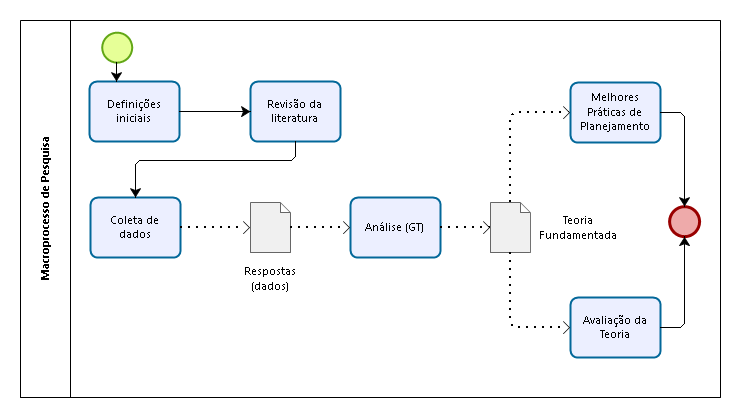
\includegraphics[width=15cm]{figuras/processoPesquisa.png}
\caption{Processo de Pesquisa}
\label{figura:processoPesquisa}
\end{figure}

Na etapa de definições iniciais, a primeira atividade consistiu na percepção e caracterização do problema de pesquisa como segue:
``Dados do TCU revelam que muitos entes da Administração Pública Federal não cumprem a determinação de realizar o planejamento da TI. Além disso, nos planos de TI dos órgãos que o fazem, são encontradas deficiências que comprometem sua eficácia. Em suma, a falta de planejamento de TI evidencia o baixo nível de maturidade em governança de TI nestas instituições.''.

Os dados do relatório do TCU que detalham o cenário que levou à formatação deste problema de pesquisa podem ser encontrados em \citeonline{tcu:14}. Apesar do relatório não revelar a identidade de cada organização, foram avaliadas entidades do poder Executivo, Judiciário, Legislativo e Ministério Público.

A partir do problema de pesquisa pôde-se definir a questão de pesquisa, como segue: ``apesar da obrigatoriedade e dos conhecidos benefícios, o planejamento de TI não é realizado satisfatoriamente nos órgãos públicos brasileiros. A atividade de planejamento envolve aspectos técnicos e sociais, diante disso, pergunta-se: quais os fatores que dificultam o processo de elaboração do planejamento de TI e qual a relação entre tais fatores?''.

Dado o problema de pesquisa, se fez necessário buscar na literatura trabalhos relacionados ao tema. Na revisão da literatura foram utilizadas as bases do Portal de Periódicos da CAPES para pesquisar trabalhos tanto na língua portuguesa quanto na língua inglesa. Os trabalhos retornados pelas \textit{strings} de busca foram filtrados através de eliminação por títulos, resumos, e por fim, eliminação após leitura completa. No capítulo final deste trabalho são apresentados os trabalhos relacionados selecionados na revisão da literatura.

Após a leitura dos trabalhos mais recentes relacionados à temática do planejamento de TI no setor público, foi possível definir o escopo do trabalho e os métodos de pesquisa. Optou-se por uma abordagem qualitativa na qual o método \textit{Grounded Theory} foi  definido como ferramenta de análise dos dados.

%@to-do: colocar uma versão do questionário nos apêndices e dar um jeito de referenciar aqui neste parágrafo.
%@to-do: vou ter que colocar as respostas das perguntas também. Mas acho que talvez seja melhor em um apêndice distinto.
Na etapa seguinte, a coleta de dados ocorreu através de um questionário disponibilizado \textit{on-line} para o público alvo: participantes da elaboração e/ou revisão de PDTI de universidades federais (UFs) e institutos federais de educação, ciência e tecnologia (IFs). Obteve-se 53 respostas de 37 instituições diferentes, sendo 20 UFs, das 63 existentes no país e 17 IFs, dos 41 existentes. Portanto, a pesquisa tem uma amostra de 35,57\% das instituições federais de ensino superior e técnico. O questionário é composto de perguntas dissertativas (qualitativas) e perguntas objetivas (quantitativas), como pode ser visto no \autoref{apendice:a_quest_coleta}.

As respostas coletadas servem como \textit{input} para a etapa de análise dos dados, cujas atividades são as fases de codificação da GT: codificação aberta, codificação axial e codificação seletiva. O resultado da etapa de análise constitui a teoria fundamentada em dados que serve de entrada para a etapa final de avaliação dos resultados.

%@to-do: verificar se quando eu falo do Likert eu devo colocar alguma nota de rodapé ou referenciar alguma obra dele
%@to-do: incluir questionário de avaliação nos apêndices
A etapa de avaliação dos resultados ocorreu por meio de questionário eletrônico com itens de \textit{Likert}, que pode ser visualizado no \autoref{apendice:b_quest_avaliacao}. Os resultados desta etapa e das etapas anteriores são pormenorizadas no Capítulo 4 deste trabalho.

A teoria resultante da análise com \textit{Grounded Theory} também serve de entrada para a etapa de seleção das melhores práticas de planejamento de TI. Nesta etapa, detalhada no Capítulo 5, executou-se novamente técnicas da \textit{Grounded Theory} com o objetivo de relacionar as melhores práticas de planejamento estratégico de TI com os elementos da teoria descoberta na análise dos dados.


\section{Princípios da Grounded Theory}
\label{secao:principios_da_gt}
O termo ``pesquisa qualitativa'' pode ser atribuído às pesquisas cujas descobertas são oriundas de métodos não estatísticos \cite{corbin:98}. De acordo com \citeonline{stern:80}, métodos qualitativos podem ser usados para explorar, de forma substancial, áreas pouco conhecidas ou para se obter um novo entendimento de uma área já conhecida. Pesquisas qualitativas podem se referir, por exemplo, a comportamentos, experiências vividas, emoções, funcionamento organizacional, movimentos sociais e fenômenos culturais \cite{corbin:98}.

A abordagem qualitativa pode ser aplicada através de diversos métodos, como a etnografia, pesquisa-ação e estudos de caso \cite{patton:90}. A definição do método a ser utilizado pode envolver diversas variáveis, como o objetivo de pesquisa, habilidades do pesquisador, participantes e os recursos a serem utilizados na pesquisa \cite{easterbrook:08}.

A proposta apresentada neste trabalho consiste na utilização do método de pesquisa qualitativa \textit{Grounded Theory}  \cite{glaser:68}, ou Teoria Fundamentada em Dados, visando elucidar o problema da elaboração de PDTI nos órgãos públicos brasileiros. Este método foi originalmente desenvolvido pelos sociólogos Barney Glaser e Anselm Strauss no fim da década de sessenta. Com o passar do tempo, os autores da GT desenvolveram pensamentos divergentes sobre aplicação do método, culminando em duas linhas de pensamento: a \textit{Grounded Theory} Glaseriana, descrita por \citeonline{glaser:92}, e a \textit{Grounded Theory} Straussiana, de \citeonline{strauss:87} consolidada com a contribuição de Juliet Corbin \cite{corbin:98}.

\citeonline{niekerk:09} pesquisaram as principais diferenças entre as duas linhas de pensamento da GT. A linha de pensamento Straussiana, vertente a ser adotada na presente pesquisa, parte do princípio que o pesquisador já possui uma questão de pesquisa a ser respondida. Ao contrário, a vertente Glaseriana diz que o pesquisador deve possuir apenas a área do problema em mente, e que a questão de pesquisa emergirá durante a própria pesquisa. Com relação à sensibilidade teórica, a linha Glaseriana conta com a habilidade do pesquisador em gerar seus próprios conceitos e propriedades a partir dos dados. Já a linha Straussiana conta com a sensibilidade do pesquisador ao atribuir significado aos conceitos presentes nos dados.

Apesar das duas vertentes, a GT pode ser definida como um método científico que utiliza um conjunto de procedimentos sistemáticos de coleta e análise dos dados para gerar, elaborar e validar teorias substantivas sobre fenômenos essencialmente sociais, ou processos sociais abrangentes \cite{bandeira:03}. Neste contexto, o termo ``teoria'' pode ser entendido como ``um conjunto de categorias bem desenvolvidas (conceitos) que estão sistematicamente inter-relacionadas através de sentenças de relacionamento (proposições) para formar o esquema teórico que explica um fenômeno social'' \cite[p. 22]{corbin:98}.

Segundo \citeonline{conte:09}, ``a essência do método \textit{Grounded Theory} é que a teoria substantiva emerge dos dados, ou seja, é uma teoria fundamentada em uma análise sistemática dos dados''. Desta forma, o resultado de uma pesquisa que utiliza GT como método traz uma teoria fiel à realidade dos dados, reduzindo a influência dos preconceitos do pesquisador \cite{bandeira:03}. Embora o objetivo da GT seja a descoberta de teorias substantivas, o pesquisador pode optar por apenas algumas das etapas ou procedimentos da GT para satisfazer seus objetivos de pesquisa \cite{corbin:98}.

De acordo com a vertente Straussiana, a GT se baseia na ideia de codificação (\textit{coding}), que é o processo de analisar os dados para identificar conceitos (ou códigos) e categorias \cite{conte:09}. Um conceito (ou código) atribui um nome a um fenômeno de interesse para o pesquisador, ou seja, abstrai um evento, objeto, ação, ou interação que tem algum significado para o pesquisador no contexto de sua pesquisa \cite{corbin:98}. As categorias são conjuntos de conceitos relacionados \cite{birks:11}. O processo de codificação pode ser dividido em três fases: codificação aberta, axial e seletiva.
 
\begin{itemize}  
\item Codificação Aberta: etapa em que o pesquisador varre o material coletado e busca extrair conceitos, categorias e suas propriedades e dimensões;
\item Codificação Axial: nesta etapa ocorre o processo de relacionar categorias entre si e entre as propriedades e dimensões. Através destes relacionamentos é possível traçar proposições acerca do fenômeno estudado;
\item Codificação Seletiva: etapa em que o pesquisador identifica a categoria central do fenômeno e realiza o refinamento da teoria que emerge dos dados.
\end{itemize}

Apesar de serem apresentadas de forma linear, as fases do processo de codificação se sobrepõem e o fluxo admite a circularidade e, por isso, devem ser melhor compreendidas como tarefas do pesquisador e não como etapas de um processo linear \cite{bandeira:03}. Na Figura \ref{figura:GTprocesso} o processo de codificação é apresentado em sua forma iterativa.

\begin{figure}[h!]
\centering % para centralizarmos a figura
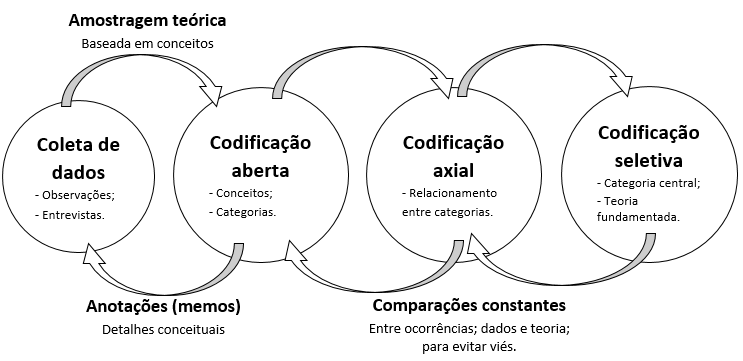
\includegraphics[width=15.5cm]{figuras/GTprocesso.png}
\caption{Processo de análise com \textit{Grounded Theory}, adaptado de \citeonline{cho:14}}
\label{figura:GTprocesso}
\end{figure}

%parágrafo da codificação aberta
A codificação aberta, ou codificação inicial, consiste no mapeamento de conceitos explorando minuciosamente os dados ao ler o material coletado de forma intensiva \cite{conte:09}. Os incidentes ou eventos são agrupados em códigos (conceitos) através da comparação incidente-incidente no intuito de gerar amostragens teóricas e ter evidências suficientes para formar categorias fundamentadas nos dados \cite{bandeira:03}. De acordo com \citeonline{cresswell:98}, durante a codificação aberta pergunta-se: o que o dado está sugerindo? Sob qual ponto de vista? Em qual categoria este dado específico se enquadra?

A codificação axial tem o objetivo de ordenar, sintetizar e organizar os códigos mapeados na codificação aberta e, principalmente, descobrir relações entre eles \cite{cresswell:98}. Neste processo pergunta-se aos dados: ``quando? Onde? Por quê? Quem? Como? Quais as consequências?'' \cite[p. 125]{corbin:98}. Nesta fase o pesquisador relaciona as categorias umas com as outras e com subcategorias, especificando suas propriedades e dimensões fundamentando os relacionamentos nos dados \cite{charmaz:14}. Na Tabela \ref{tabela:conectores} são apresentados os conectores utilizados para caracterizar relacionamentos entre códigos.

\begin{table}[h!]
\centering
\resizebox{\textwidth}{!}{%
\begin{tabular}{|l|l|}
\hline
\rowcolor[HTML]{9B9B9B} 
\textbf{Rótulo} & \textbf{Descrição do relacionamento} \\ \hline
is a & \begin{tabular}[c]{@{}l@{}}O código-origem é um tipo, ou forma, do código-destino encontrada nos \\ dados, e possui um padrão determinado de variação dimensional ao longo\\ das propriedades da categoria (código destino)\end{tabular} \\ \hline
is cause of & O código-origem (condição causal) causa a ocorrência do código-destino \\ \hline
is part of & \begin{tabular}[c]{@{}l@{}}O código-origem é uma parte, que compõe juntamente com outras partes o \\ código destino\end{tabular} \\ \hline
is associated with & \begin{tabular}[c]{@{}l@{}}Os códigos possuem uma ligação entre si que não pôde ser classificada \\ como algum dos relacionamentos anteriores\end{tabular} \\ \hline

\end{tabular}%
}
\caption{Conectores de códigos, adaptado de \citeonline{bandeira:03}}
\label{tabela:conectores}
\end{table}

A terceira e última fase de codificação, chamada de codificação seletiva, tem o objetivo de integrar e refinar as categorias para que, desta forma, seja possível identificar a categoria central do fenômeno pesquisado \cite{corbin:98}. Nesta fase grande parte dos dados foram codificados, as relações entre categorias identificadas e o pesquisador tem condições de inferir a categoria que consegue integrar as demais \cite{bandeira:03}. Notas e diagramas feitos durante as análises podem auxiliar o pesquisador na descoberta da teoria central.



\section{Grounded Theory no Contexto da Pesquisa}
%pq foi escolhida para meu problema
Abordagens quantitativas são muito úteis no sentido de prover indicadores. Porém, restringir a identificação das causas que levaram a obtenção destes indicadores à análise quantitativa pode omitir aspectos relevantes do comportamento dos indivíduos cuja influência não pode ser desprezada \cite{conte:09}. Desta forma, métodos qualitativos são indicados quando busca-se compreender, de forma mais abrangente, todo o fenômeno em estudo ao invés de simplesmente simplificar e produzir similaridades \cite{seaman:99}. Uma vantagem em utilizar métodos qualitativos de pesquisa é a necessidade de o pesquisador se aprofundar na complexidade do problema, ao invés de abstraí-la. Isto resulta em dados mais ricos e mais informativos \cite{seaman:08}.

O problema de pesquisa é o ponto de partida que origina questões de pesquisa abertas, gerais e não formalizadas a priori na forma de hipóteses específicas e fechadas \cite{bandeira:03}. Considerando que (i) a questão de pesquisa deste trabalho não forma uma hipótese específica, ou seja, trata-se de uma questão aberta; (ii) considerando que existem trabalhos com abordagens quantitativas acerca do problema desta pesquisa e que, portanto, podem omitir aspectos relevantes do comportamento humano; (iii) considerando que o objetivo principal desta pesquisa busca compreender um fenômeno de forma abrangente; tem-se um cenário apto para a abordagem qualitativa aplicando o método \textit{Grounded Theory} para responder a questão de pesquisa. 

Portanto, nesta pesquisa a \textit{Grounded Theory} atua como ferramenta fundamental na proposta de identificar e compreender os fatores que dificultam o planejamento de TI em instituições públicas federais. O principal aspecto da abordagem desta pesquisa consiste na formulação de uma teoria fundamentada em dados para o problema do planejamento de TI, ou seja, ao aplicar a GT, os resultados são fiéis à realidade refletida nos dados coletados com os envolvidos na temática estudada, ao contrário de outros métodos que dependem da interpretação do pesquisador. 

De posse dos resultados da aplicação da GT espera-se, como consequência desta pesquisa, propor um conjunto de melhores práticas de planejamento que atinjam as causas encontradas neste trabalho. Tais causas são os elementos da teoria que emerge dos dados que possuem relação de causa com o problema pesquisado, por exemplo, se uma das causas do problema é ``falta de capacitação", então espera-se encontrar um conjunto de melhores práticas cujos resultados minimizem o este elemento causal. Desta forma, é pretendido oferecer um meio de, eventualmente, melhorar os índices de planejamento de TI nas instituições pesquisadas. 

\section{Considerações}
Este capítulo apresentou uma visão geral do processo de pesquisa definido para este trabalho, desde as definições iniciais, coleta de dados, análise com GT, até as atividades de avaliação dos resultados. Dois pontos relevantes, sob a perspectiva metodológica, são: a abordagem qualitativa em um cenário que, tradicionalmente, é avaliado de forma quantitativa; a utilização de 
\textit{Grounded Theory} como método para apoiar na compreensão do fenômeno estudado. 

Há de se destacar que esta pesquisa tem um caráter multidisciplinar, pois abrange não somente a área de tecnologia da informação, mas também aspectos da administração e sociologia, uma vez que visa compreender o comportamento dos indivíduos envolvidos em atividades de gestão em um ambiente regido pela TI. Neste cenário a \textit{Grounded Theory} se torna determinante para compreender os fatores sociotécnicos envolvidos no planejamento de TI. No capítulo seguinte, é apresentado o referencial teórico com os principais conceitos inerentes à temática da pesquisa.